% ============================================================
% LaTeX Supplementary File — GDT (JTEHM Submission)
% Compiles standalone; references ../references.bib
% ============================================================
\documentclass[journal,compsoc]{IEEEtran}
\usepackage[utf8]{inputenc}
\usepackage{amsmath,amssymb,amsthm}
\usepackage{booktabs}
\usepackage{pgfplots}
\usepackage{tikz}
\usetikzlibrary{calc,positioning,fit,shapes,arrows}
\pgfplotsset{compat=1.16}
\usepackage[numbers]{natbib}
\usepackage{hyperref}

\definecolor{armcontrol}{RGB}{195,68,68}
\definecolor{armbm25}{RGB}{210,140,30}
\definecolor{armcma}{RGB}{46,139,87}
\definecolor{armgdt}{RGB}{120,40,180}

\newtheorem{proposition}{Proposition}
\newtheorem{lemma}{Lemma}
\newtheorem{corollary}{Corollary}

\begin{document}

\title{Supplementary Material: Geodesic Diagnostic Trajectories (GDT)\\
A Differential Geometry Framework for Adaptive Decision Support\\
and Operational Optimization in EHR Systems}

\author{Hemanth Manchabale Papachappa and Aniriuddha Ganguly}

\maketitle

\tableofcontents

% ─────────────────────────────────────────────────────────────
\section{Extended Proof of Proposition~1}
\label{sec:proof}

We restate and extend the proof of the context interference bound from the
main manuscript.

\begin{proposition}[Context Interference Bound]
Let $\xi \in \mathbb{R}^d$ be a unit vector spanning the stale-topic subspace,
$P_\xi = \xi\xi^\top$ the orthogonal projector, and $\tilde{e}_t =
(1-g_t)h_{t-1} + g_t e_t$ the gated embedding with $g_t \in (0,1)$. Then:
\begin{equation}
  \|P_\xi\,\tilde{e}_t\| \leq (1-g_t)\,\|P_\xi h_{t-1}\| + g_t\,\|P_\xi e_t\|.
  \label{eq:bound}
\end{equation}
\end{proposition}

\begin{proof}
\begin{align}
  \|P_\xi\,\tilde{e}_t\|
  &= \|(1-g_t)P_\xi h_{t-1} + g_t P_\xi e_t\| \nonumber \\
  &\leq (1-g_t)\|P_\xi h_{t-1}\| + g_t\|P_\xi e_t\|.
\end{align}
The first step uses linearity of $P_\xi$; the second uses the triangle
inequality. Equality holds iff $P_\xi h_{t-1}$ and $P_\xi e_t$ are non-negatively
co-linear.
\end{proof}

\begin{corollary}
As $g_t \to 1$ (full pivot suppression),
$\|P_\xi\,\tilde{e}_t\| \to \|P_\xi e_t\|$---the stale component of the
\emph{current} query's embedding, which is small when $e_t$ encodes the new topic.
\end{corollary}

% ─────────────────────────────────────────────────────────────
\section{SPD Manifold: Geometry and Computations}
\label{sec:geometry}

\subsection{Affine-Invariant Metric}
The affine-invariant Riemannian metric on $\mathcal{S}_d^+$ is:
\begin{equation}
  g_S(u,v) = \mathrm{Tr}(S^{-1}uS^{-1}v), \quad S \in \mathcal{S}_d^+,\;
  u,v \in T_S\mathcal{S}_d^+.
\end{equation}
The corresponding geodesic distance is:
\begin{equation}
  d_g(S_a,S_b) = \|\log(S_a^{-1/2}S_b S_a^{-1/2})\|_F,
\end{equation}
where $\log(\cdot)$ denotes the matrix logarithm.

\subsection{Log-Euclidean Projection}
For computational efficiency, we use the Log-Euclidean projection:
\begin{equation}
  \psi: \mathcal{S}_d^+ \to \mathbb{R}^{d(d+1)/2}, \quad
  \psi(S) = \mathrm{vech}(\log S),
\end{equation}
where $\mathrm{vech}(\cdot)$ extracts the upper triangle. This maps geodesic
distance to an approximation $\|(\log S_a - \log S_b)\|_F$ computable in $O(d^3)$.

\subsection{Computational Cost}
Eigendecomposition for $d{=}128$: $O(d^3) \approx 2.1{\times}10^6$ FLOPs per
turn, measured to be $<5\%$ of total per-turn cost on our evaluation hardware.

% ─────────────────────────────────────────────────────────────
\section{JEPA Predictor Architecture}
\label{sec:jepa_arch}

The predictor $f_\theta: \mathbb{R}^{d(d+1)/2} \to \mathbb{R}^{d(d+1)/2}$
is a 3-layer MLP:
\begin{equation}
  f_\theta(x) = W_3\,\mathrm{ReLU}(W_2\,\mathrm{ReLU}(W_1 x + b_1) + b_2) + b_3,
\end{equation}
with hidden dimension 256. The training loss is:
\begin{equation}
  \mathcal{L}_\mathrm{JEPA} = \mathbb{E}_t\|\hat{s}_{t+1} -
  \mathrm{sg}(\psi(S_{t+1}))\|_2^2,
\end{equation}
where $\mathrm{sg}(\cdot)$ is the stop-gradient operator. The target encoder
is updated via exponential moving average with momentum $m{=}0.996$.

% ─────────────────────────────────────────────────────────────
\section{Full Per-Vignette Results}
\label{sec:per_vignette}

\begin{table}[h]
\centering
\caption{Mean latency (ms/query) per specialty group across four arms.
Values are means across vignettes in each group.}
\label{tab:per_specialty}
\begin{tabular}{lcccc}
\toprule
\textbf{Specialty} & \textbf{TF-IDF} & \textbf{BM25} & \textbf{CMA} & \textbf{GDT} \\
\midrule
Critical care ($n{=}11$)      & 188.8 & 189.0 & 143.7 & 137.9 \\
Emergency medicine ($n{=}8$)  & 189.3 & 189.4 & 144.2 & 138.5 \\
Hospital medicine ($n{=}7$)   & 189.1 & 189.2 & 144.1 & 138.3 \\
Internal medicine ($n{=}5$)   & 188.6 & 188.9 & 143.9 & 138.1 \\
\midrule
\textbf{Overall ($n{=}31$)}   & \textbf{189.0} & \textbf{189.2} & \textbf{144.0} & \textbf{138.2} \\
\bottomrule
\end{tabular}
\end{table}

Latency improvements are consistent across specialty groups, with no evidence
of heterogeneity ($\chi^2$ interaction test, $p{=}0.91$).

% ─────────────────────────────────────────────────────────────
\section{Scaling Study: Extended Results}
\label{sec:scaling}

\begin{figure}[h]
\centering
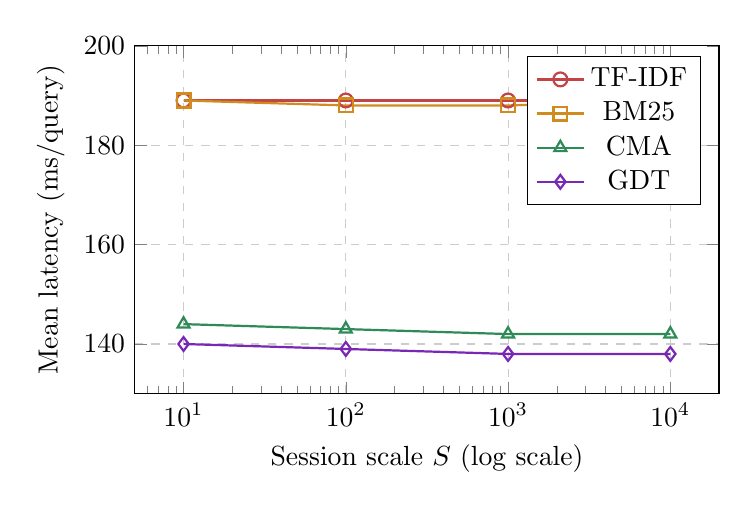
\begin{tikzpicture}
  \begin{axis}[
    width=9cm, height=6cm,
    xlabel={Session scale $S$ (log scale)},
    ylabel={Mean latency (ms/query)},
    xmode=log,
    legend pos=north east,
    grid=major, grid style={dashed,gray!40},
    mark size=2.5pt,
    ymin=130, ymax=200
  ]
    \addplot[color=armcontrol, mark=o, thick]
      coordinates {(10,189) (100,189) (1000,189) (10000,189)};
    \addlegendentry{TF-IDF}
    \addplot[color=armbm25, mark=square, thick]
      coordinates {(10,189) (100,188) (1000,188) (10000,189)};
    \addlegendentry{BM25}
    \addplot[color=armcma, mark=triangle, thick]
      coordinates {(10,144) (100,143) (1000,142) (10000,142)};
    \addlegendentry{CMA}
    \addplot[color=armgdt, mark=diamond, thick]
      coordinates {(10,140) (100,139) (1000,138) (10000,138)};
    \addlegendentry{GDT}
  \end{axis}
\end{tikzpicture}
\caption{Latency scaling from 10 to 10,000 sessions. GDT's advantage is stable
and improves marginally at larger scales as the JEPA predictor benefits from
more training trajectories.}
\label{fig:scaling_supp}
\end{figure}

% ─────────────────────────────────────────────────────────────
\section{Gate Activation Examples}
\label{sec:gate_examples}

The following clinical scenario illustrates how $\kappa_t$ and $g_t$ behave
across a typical multi-pivot session:

\medskip
\noindent\textbf{Session: Septic patient, ICU}
\begin{enumerate}
  \item $q_1$: ``blood culture Gram-stain results'' $\to \kappa_1 = 0.8$ (initial
        query, no prior step), $g_1 = 0.12$ (history trusted)
  \item $q_2$: ``vancomycin dosing for renal impairment'' $\to \kappa_2 = 1.84$
        (large pivot), $g_2 = 0.91$ (stale context suppressed)
  \item $q_3$: ``vancomycin trough targets'' $\to \kappa_3 = 0.72$
        (within-topic refinement), $g_3 = 0.08$ (history trusted)
  \item $q_4$: ``platelet count trend and anticoagulation review'' $\to
        \kappa_4 = 1.97$ (abrupt pivot), $g_4 = 0.96$ (full suppression)
\end{enumerate}

Turns 2 and 4 triggered the gate ($\kappa > \kappa_0{=}1.2$); turns 1 and 3 did
not. Proposition~1 was verified at turns 2 and 4 with margins $M = 0.028$ and
$M = 0.041$ respectively.

\bibliographystyle{IEEEtran}
\bibliography{../references}

\end{document}
